\renewcommand{\theequation}{\theenumi}
\begin{enumerate}[label=\arabic*.,ref=\thesubsection.\theenumi]
\numberwithin{equation}{enumi}
\item total no of bages = 5\\
No of bages having 40 germinated seeds = 3\\

probability of a bag having 40 germinated seeds  = P(X=40)
\\
\begin{align}
P\left(X=40\right) &= \frac{3}{5}
\\
&= 0.6
\end{align}

No of bages having 49 germinated seeds = 0\\

probability of a bag having 49 germinated seeds  = P(X=49)
\\
\begin{align}
P\left(X=49\right) &= \frac{0}{5}
\\
&= 0
\end{align}
No of bages having more than 35 germinated seeds = 5\\

probability of a bag having more than 35 germinated seeds  = $P(X>35)$
\
\begin{align}
P\left(X>35\right) &= \frac{5}{5}
\\
&= 1
\end{align}
codes for the above equation can be get from here
\begin{lstlisting}
codes/probexm/probexm10.py
\end{lstlisting}
\begin{figure}[!ht]
	\centering
	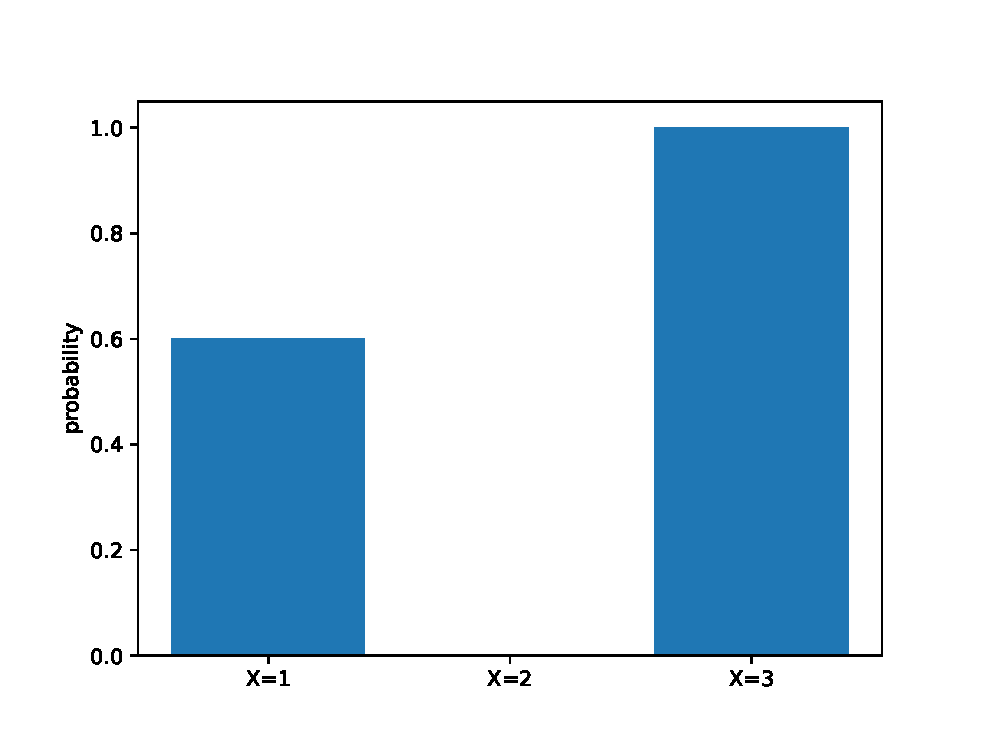
\includegraphics[width=\columnwidth]{./figures/probexm/probexm10.eps}
	\caption{probability of germinated seeds in a bag }
	\label{fig:bt10}
	\begin{lstlisting}
	figs/probexm/probexm10.eps
	\end{lstlisting}
\end{figure}
\end{enumerate}